\chapter{Introducción específica} % Main chapter title

\label{Chapter2}

%----------------------------------------------------------------------------------------
%	SECTION 1
%----------------------------------------------------------------------------------------
En este capítulo se describen las tecnologías y los protocolos de comunicación, los componentes de hardware, las herramientas de software y los requerimientos para la realización del proyecto.

\section{Tecnologías de comunicación}
\label{sec:Tecnologías de comunicación}
Los principales protocolos de IoT empleados en el trabajo son: MQTT \citep{mqtt}, HTTP \citep{rfc1057}, SSL/TLS \citep{tls:1} e IEEE 802.11 \citep{802.11}. 
Según el modelo TCP/IP \citep{rfc1180} los tres primeros se encuentran en la capa de aplicación mientras que el cuarto se ubica en la capa de enlace. Esto se esquematiza en la figura \ref{fig:IotProtocols}.

%A continuación se describen los principales protocolos empleados en el trabajo. En la figura \ref{fig:IotProtocols} se observa su posicionamiento en la pila de protocolos para IoT.

\begin{figure}[h]
	\centering
	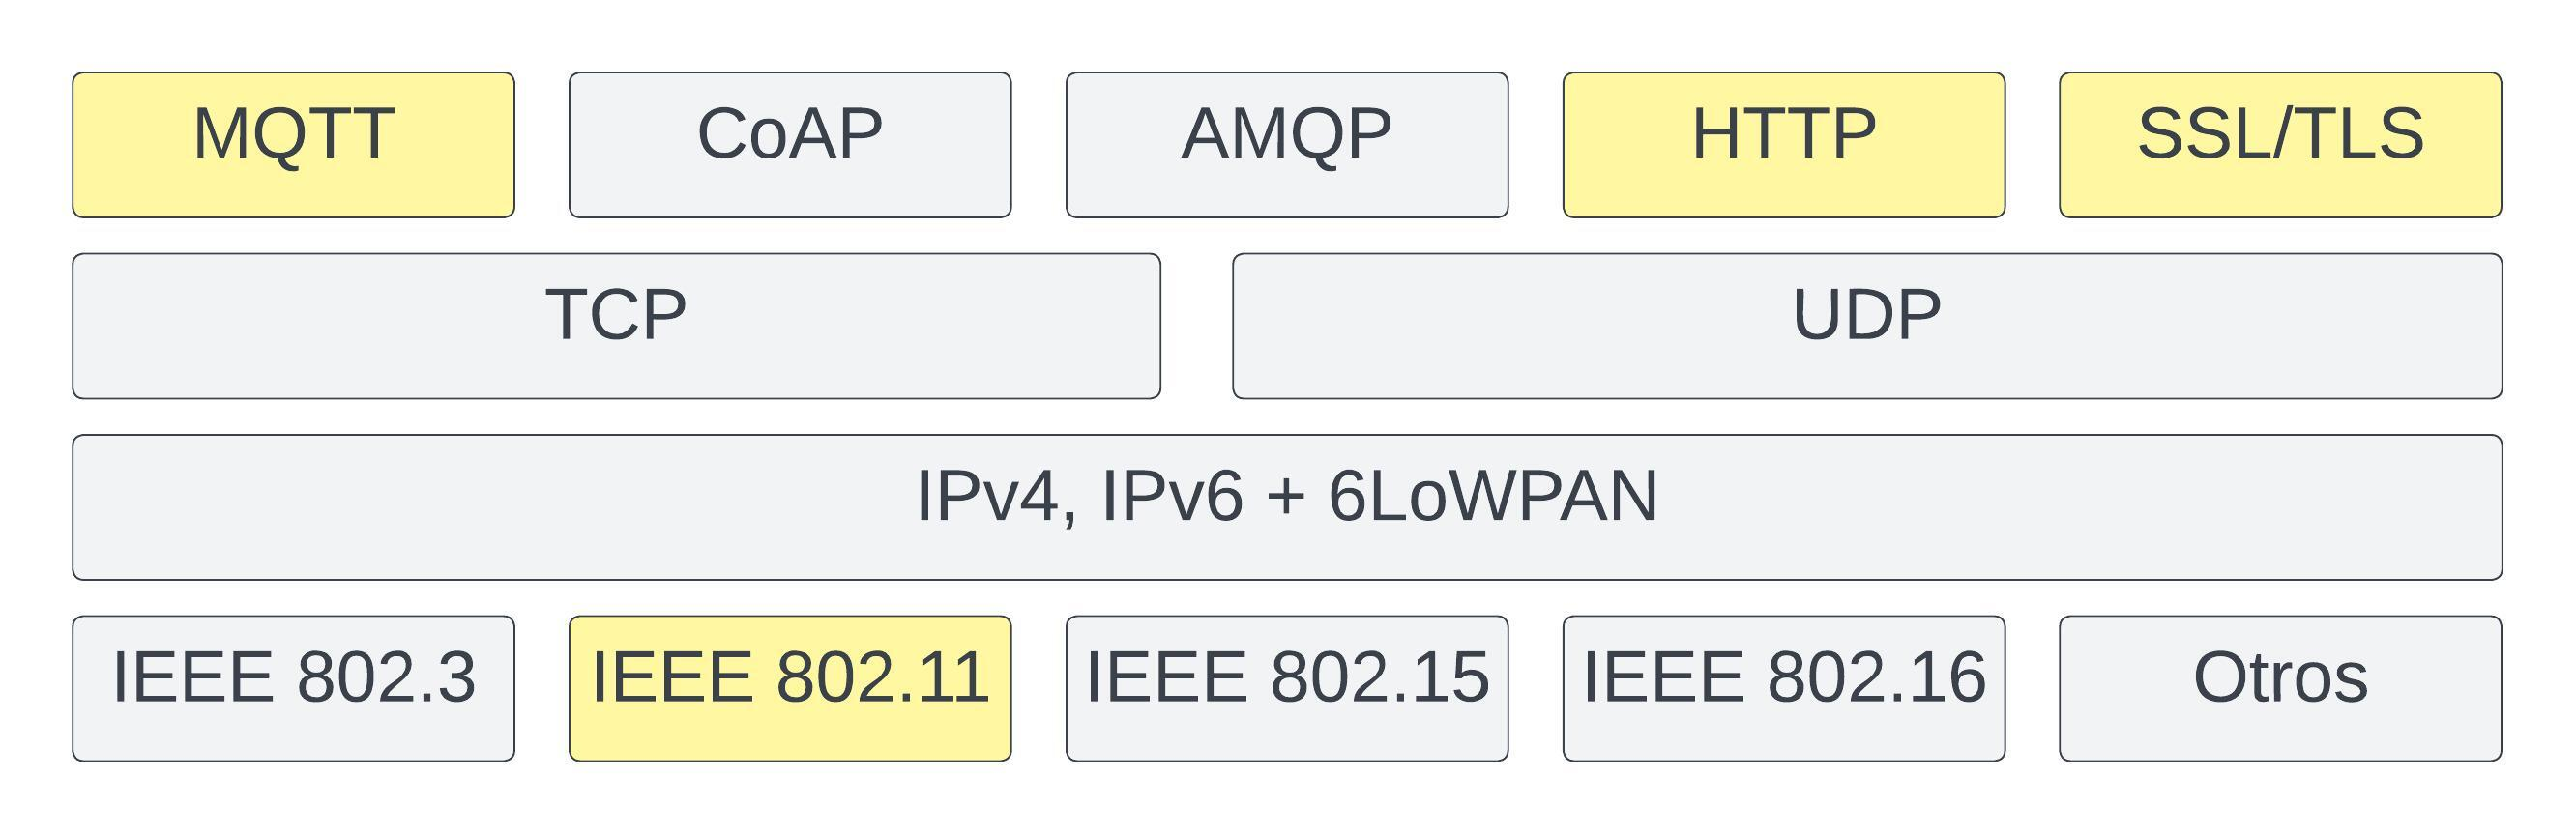
\includegraphics[width=0.75\textwidth]{./Figures/protocols.jpeg}
	\caption[Ubicación de los protocolos de IoT en la pila TCP/IP]{Ubicación de los protocolos de IoT en la pila TCP/IP.}
	\label{fig:IotProtocols}

\end{figure}
	



\subsection{Protocolo MQTT}
\label{sec:Protocolo MQTT}

MQTT fue desarrollado en 1999 con el objetivo principal de crear un protocolo muy eficiente desde el punto de vista del uso del ancho de banda y de muy bajo consumo de energía. Por estas razones es ampliamente utilizado en IoT \citep{mqtt:1}.

Su funcionamiento se basa en el paradigma de publicación-suscripción \citep{pubsub}, el cual consiste en desvincular un cliente que publica un mensaje (publicador) de otros clientes que reciben el mensaje (suscriptores). Otra característica importante a mencionar es que, al ser un protocolo asincrónico, el cliente puede seguir operando mientras espera un nuevo mensaje.


%Se basa en el paradigma de publicación-suscripción \citep{pubsub}, donde el agente que publica un mensaje (publicador) no mantiene ningún vínculo directo con otros clientes que reciben el mensaje (suscriptores). Por tratarse de un protocolo asincrónico, los clientes pueden seguir operando mientras esperan un nuevo mensaje.



Un componente principal del protocolo es el \textit{broker} cuya función primaria es la de recibir los mensajes de los publicadores y enviarlos a los  suscriptores. Para realizar esta tarea, el \textit{broker} utiliza temas o \textit{topics} para agrupar clientes que necesitan recibir los mismos mensajes. De esta manera el \textit{topic} es un canal virtual que conecta a los publicadores con sus suscriptores \citep{mqtt:1}.

En la figura \ref{fig:arqmqtt} se observa la arquitectura del protocolo.
\begin{figure}[h]
	\centering
	\includegraphics[width=0.90\textwidth]{./Figures/mqtt.jpeg}
	\caption[Arquitectura del protocolo MQTT]{Arquitectura del protocolo MQTT.}
	\label{fig:arqmqtt}

\end{figure}




\subsection{Protocolo HTTP}
\label{sec:Protocolo HTTP}

El \textit{Hypertext Transfer Protocol} (HTTP)\citep{http:1} es un protocolo utilizado en la Web para el desarrollo de aplicaciones y está basado en el paradigma cliente-servidor. Aquí el cliente emplea un agente intermediario (por lo general un \textit{browser}) para realizar un pedido de información y el servidor proporciona una respuesta. Esto se conoce con el nombre de modelo \textit{request/response}.

HTTP es un protocolo que no guarda información de estado, esto significa que el servidor no es capaz de reconocer la relación entre múltiples pedidos de un mismo usuario  \citep{oreilly:1}.

En la actualidad, HTTP se utiliza en conjunto con la arquitectura REST (\textit{Representational State Transfer}) \citep{rest} para facilitar la interacción entre distintas entidades sobre servicios basados en red. Esta asociación permite que los dispositivos interactúen mediante funciones estándares de tipo CRUD (\textit{create, read, update, delete})  \citep{10.1145/3292674}. Dichas funciones a su vez se traducen en los métodos HTTP POST, GET, PUT y DELETE respectivamente \citep{GLAROUDIS2020107037}. 


\subsection{Protocolo SSL/TLS}
\label{sec:Protocolo SSL/TLS}
\textit{Secure Socket Layer/Transport Layer Security} (SSL/TLS) es un protocolo criptográfico que proporciona seguridad de extremo a extremo de los datos enviados entre aplicaciones a través de Internet.
TLS evolucionó a partir de \textit{Secure Socket Layer} (SSL), que fue desarrollado originalmente por Netscape Communications Corporation en 1994 para proteger las sesiones web. 

%SSL 1.0 nunca se lanzó públicamente, mientras que SSL 2.0 fue reemplazado rápidamente por SSL 3.0 que proporcionó las bases para la posterior creación de TLS. 

Cabe señalar que TLS no protege los datos en los sistemas finales, simplemente garantiza la entrega segura de datos a través de Internet y al mismo tiempo evita posibles escuchas y/o alteraciones del contenido.
TLS normalmente se implementa sobre TCP \citep{rfc793} para cifrar los protocolos de la capa de aplicación, como por ejemplo HTTP.

TLS utiliza una combinación de criptografía simétrica y asimétrica que proporciona un buen compromiso entre rendimiento y seguridad al momento de transmitir la información \citep{tls:2}. Para mayor protección es deseable que un cliente que se conecta a un servidor pueda validar la veracidad de la clave pública ofrecida por este. Normalmente dicha verificación se lleva a cabo por medio de un certificado digital X.509 \citep{x509:1} emitido por un tercero de confianza denominado Autoridad Certificadora (CA). Dicha CA está encargada de  afirmar la autenticidad de la clave pública. En los casos en los que no se dispone de una CA, un servidor puede usar un certificado autofirmado en el que el cliente debe confiar explícitamente \citep{tls:2}.


En la figura \ref{fig:ssl2way} se detalla el esquema de autenticación y verificación con certificados e inicio de una conexión segura.

\begin{figure}[h]
	\centering
	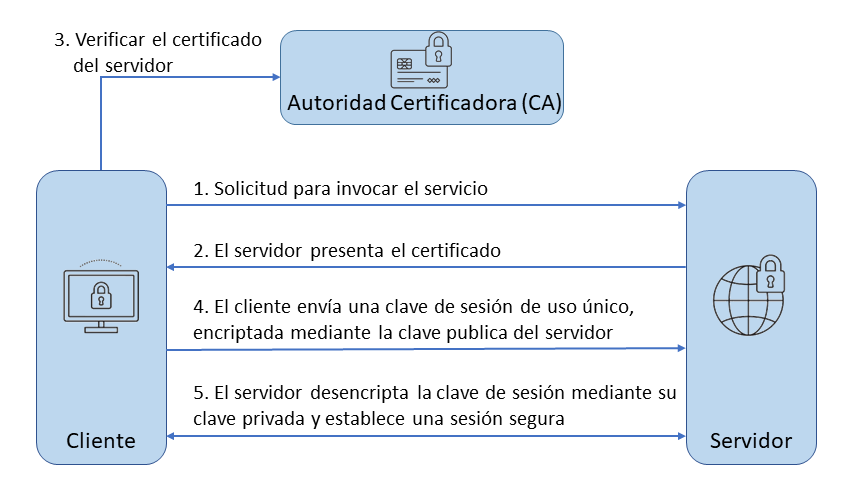
\includegraphics[width=0.9\textwidth]{./Figures/tls.png}
	\caption[Proceso de autenticación de TLS]{Proceso de autenticación de TLS\protect\footnotemark.}
	\label{fig:ssl2way}

\end{figure}
	\footnotetext{Gráfico creado en base a una imagen tomada de http://www.herongyang.com/PKI/HTTPS-Communication-Data-Encryption.html}

\subsection{Tecnologías Wi-Fi}
\label{sec:Tecnologías Wi-Fi}
El estándar IEEE 802.11 para redes inalámbricas de área local (WLAN) es conocido comercialmente como Wi-Fi y presenta dos modos de operación \citep{wifi}:
\begin{itemize}
\item Infraestructura: uno o más \textit{access points} (AP) actúan como puente entre la red cableada y la red inalámbrica. Todas las comunicaciones entre los dispositivos conectados a la red se realizan a través de los APs. 
\item Ad-hoc: cada nodo puede realizar una conexión directa con otro, sin necesidad de un AP central. En este caso, los nodos se organizan en una red donde todos son capaces de enrutar los paquetes.  
\end{itemize}

\section{Componentes de hardware utilizado}
\label{sec:Hardware utilizado}

\subsection{Raspberry Pi}
\label{sec:Raspberry Pi}
Se denomina así a una serie de computadoras monoplaca o computadoras de placa simple (SBC, por \textit{Single Board Computer}) de bajo costo desarrolladas por la Raspberry Pi Foundation \citep{raspberrypi:1}.
Una de sus principales características es proveer un conjunto de pines de GPIO (\textit{general purpose input/output}) que permiten controlar componentes electrónicos y otros dispositivos en el ámbito de Internet de las Cosas.
A pesar de su reducido tamaño, la Raspberry Pi ofrece una capacidad de procesamiento comparable a una computadora de escritorio y es por ello que su uso se ha expandido en proyectos que incluyen domótica, \textit{edge computing} y aplicaciones industriales \citep{raspberrypi:2}. 

En la figura \ref{fig:rpi} se muestra una Raspberry Pi modelo 4B similar a la utilizada en el trabajo y en la tabla \ref{tab:raspberrypi} se listan sus principales características: 
 
%\begin{table}[h]
%\centering
%\caption[Especificaciones técnicas de la Raspberry Pi 4B]{Especificaciones técnicas de la Raspberry Pi 4B.}
%
%\begin{tabular}{p{2.5cm} p{7.5cm} } 
%\toprule
%\textbf{Categoría} & \textbf{Especificación}\citep{rpi4b}\\
%
%\midrule
%Procesador	& Broadcom BCM2711, quad-core Cortex-A72 (ARM v8) 64 bits SoC @ 1,8 GHz \\
%Memoria SDRAM	 & 1, 2, 4 u 8 GB LPDDR4-3200 \\
%Wi-Fi	& 2,4 GHz y 5,0 GHz IEEE 802.11ac \\
%Bluetooth	&  5.0 y BLE \\
%Ethernet	& Gigabit, con soporte opcional para POE\\
%USB	& 2 puertos  3.0 y 2 puertos 2.0\\
%GPIO	&	Conector de 40 pines\\
%HDMI	&  2 puertos micro-HDMI\\
%Alimentación	& 5 V USB y GPIO\\
%Temperatura de operación	& 0 °C a 50 °C \\
%\bottomrule
%\hline
%\end{tabular}
%\label{tab:raspberrypi}
%\end{table}



\begin{table}[htbp]
    \centering
	\caption[Especificaciones técnicas de la Raspberry Pi 4B]{Especificaciones técnicas de la Raspberry Pi 4B.}


%\begin{tblr}{
% column{1}={0.30\textwidth}, column{2}={0.65\textwidth},
% rowsep=3pt,
% hline{1} = {0.8pt,solid}, 
% hline{2} = {0.6pt,solid}, 
% hline{12} = {1.3pt,solid},
% colspec = {X[l]X[l]},
% row{1} = {font=\bfseries}, rowhead = 1,
% } 
\begin{tblr}{
 column{1}={0.33\textwidth}, column{2}={0.55\textwidth},
 rowsep=2pt,
 hline{1} = {0.85pt,solid}, 
 hline{2} = {0.6pt,solid}, 
 hline{12} = {1.2pt,solid},
 colspec = {X[l]X[l]},
 row{1} = {font=\bfseries}, rowhead = 1,
 }
Categoría	& Especificación\citep{rpi4b}\\
Procesador	& Broadcom BCM2711, quad-core Cortex-A72 (ARM v8) 64 bits SoC @ 1,8 GHz \\
Memoria SDRAM	 & 1, 2, 4 u 8 GB LPDDR4-3200 \\
Wi-Fi	& 2,4 GHz y 5,0 GHz IEEE 802.11ac \\
Bluetooth	&  5.0 y BLE \\
Ethernet	& Gigabit, con soporte opcional para POE\\
USB	& 2 puertos  3.0 y 2 puertos 2.0\\
GPIO	&	Conector de 40 pines\\
HDMI	&  2 puertos micro-HDMI\\
Alimentación	& 5 V USB y GPIO\\
Temperatura de operación	& 0 °C a 50 °C \\

\end{tblr}
    \label{tab:raspberrypi}
\end{table}
 
\begin{figure}[h]
	\centering
	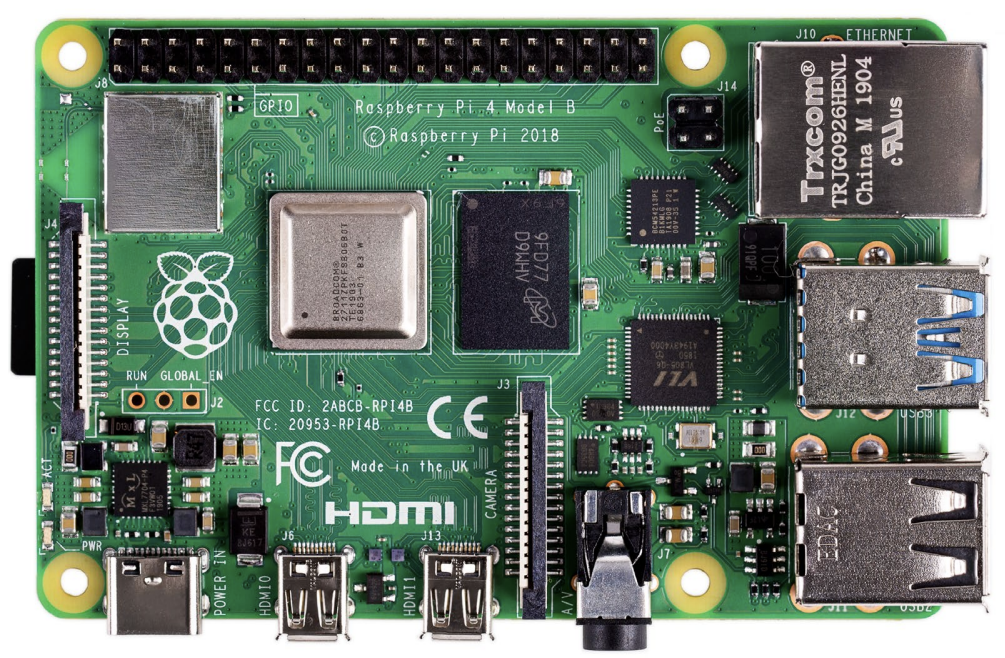
\includegraphics[width=0.55\textwidth]{./Figures/rpi.png}
	\caption[Raspberry Pi]{Raspberry Pi\protect\footnotemark.}
	\label{fig:rpi}

\end{figure}
\footnotetext{Imagen tomada de https://datasheets.raspberrypi.com/.}
\subsection{Módulos ESP}
\label{sec:Módulos ESP}
ESP es una familia de microcontroladores de baja potencia  desarrollada por la empresa china Espressif. Estos chips cuentan con una amplia variedad de usos en IoT tanto en el ámbito profesional o industrial como en el de los aficionados \citep{esp32} \citep{esp8266}. 

En la tabla \ref{tab:esp} se observa una comparación entre los modelos ESP32-WROOM-32 y ESP8266 utilizados en este trabajo.





\begin{table}[h]
\centering
\caption[Especificaciones de los microcontroladores ESP]{Especificaciones de los microcontroladores ESP.}

\begin{tabular} {p{4.5cm} p{3.7cm} p{3.7cm}} 
\toprule
\textbf{Características} & \textbf{ESP32} \citep{esp32}  & \textbf{ESP8266} \citep{esp8266} \\
\midrule
Procesador		& 2 x Xtensa 32 bits LX6	& Tensilica L106 32 bits\\
Memoria ROM	 	& 448 KB	& No dispone\\	
Memoria SRAM	& 520 KB	& 160 KB\\
Wi-Fi			& 802.11 b/g/n & 802.11 b/g/n\\
Bluetooth		& 4.2, BLE & No dispone\\
GPIOs			& 34 pines & 17 pines\\
Consumo normal	& \textasciitilde 500 mA & \textasciitilde 80 mA \\
Temperatura de operación		& -40 °C a 85 °C & -40 °C a 125 °C \\
Sistema operativo &	freeRTOS	& freeRTOS \\
Costo en USD	& \$ 6 a \$ 12  & \$ 3 a  \$ 6 \\
\bottomrule
\hline
\end{tabular}
\label{tab:esp}
\end{table}

%El modelo ESP8266 es una versión anterior al ESP32 y ofrece una menor variedad de características. Sin embargo, constituye una opción económica cuando los requerimientos de conectividad y rendimiento van de la mano con sus prestaciones.

El modelo ESP8266 es una versión anterior y con menores prestaciones que el ESP32. Constituye una opción económica para soluciones en las que los requerimientos de conectividad, cantidad de periféricos y demandas computacionales no son tan exigentes.

En la figura \ref{fig:esp32} se observa un módulo de desarrollo de la familia ESP32, mientras que el ESP8266 puede verse en la figura \ref{fig:esp8266}. 


\begin{figure}[!htpb]
     \centering
     \begin{subfigure}[b]{0.45\textwidth}
		\centering
		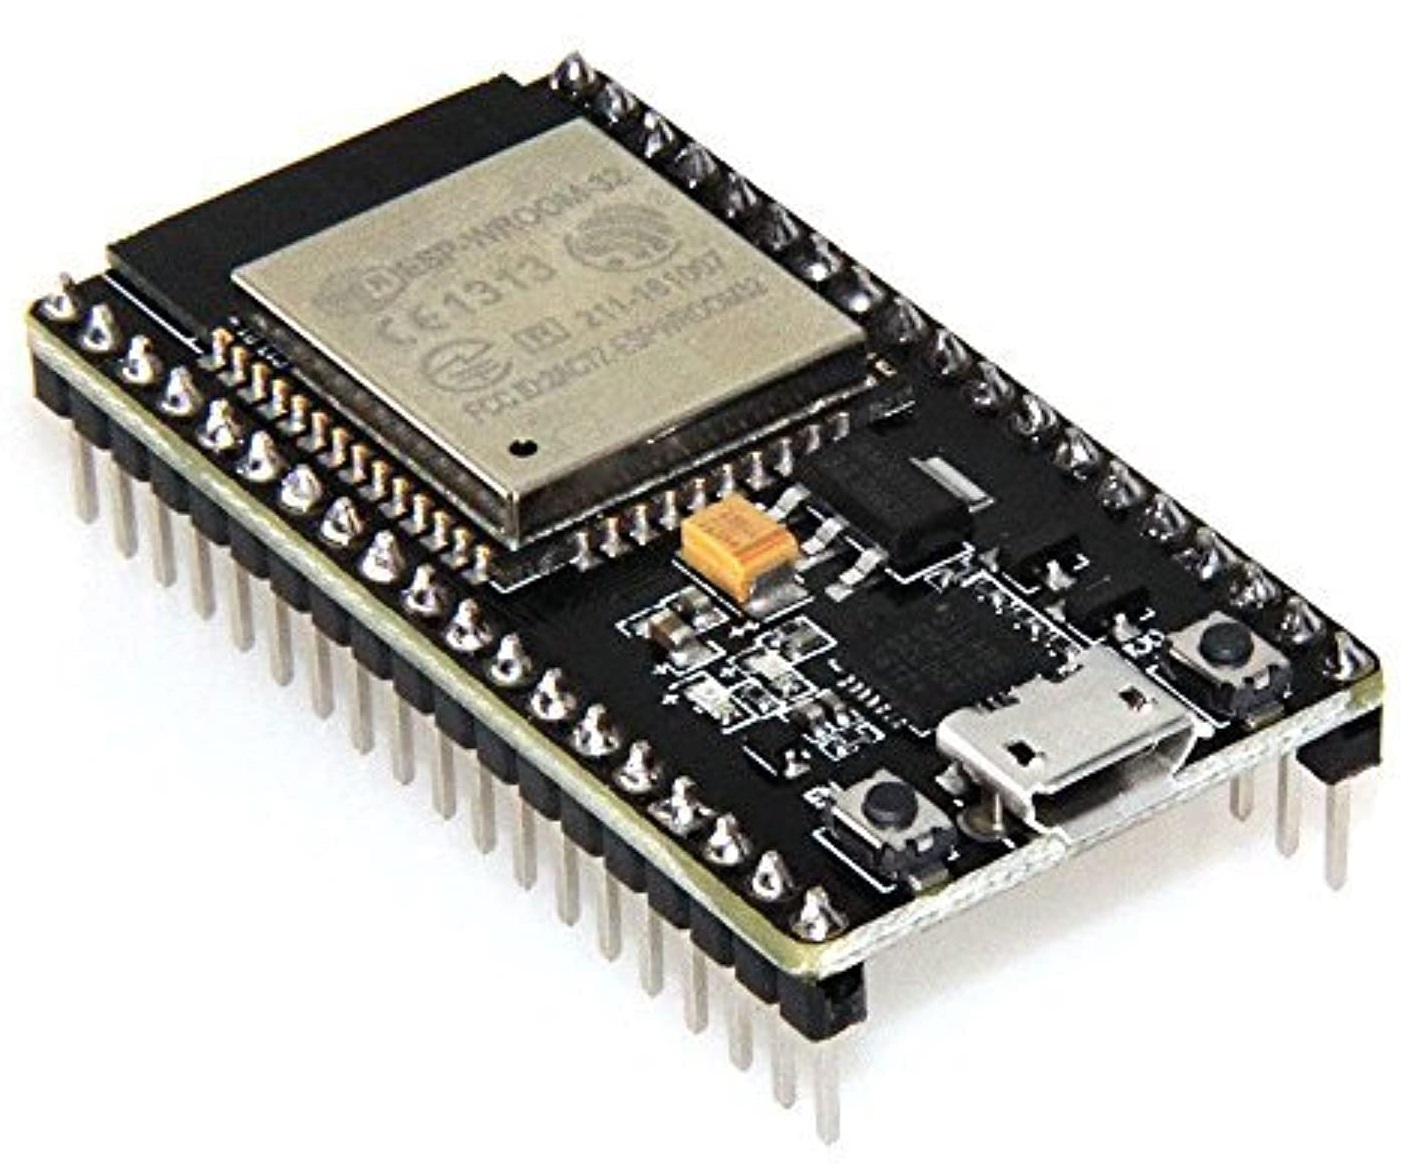
\includegraphics[width=0.60\textwidth]{./Figures/esp32.jpg}
		\caption[Módulo de desarrollo ESP32]{Módulo de desarrollo ESP32.}
		\label{fig:esp32}
     \end{subfigure}
     \hfill
     \begin{subfigure}[b]{0.45\textwidth}
	\centering
		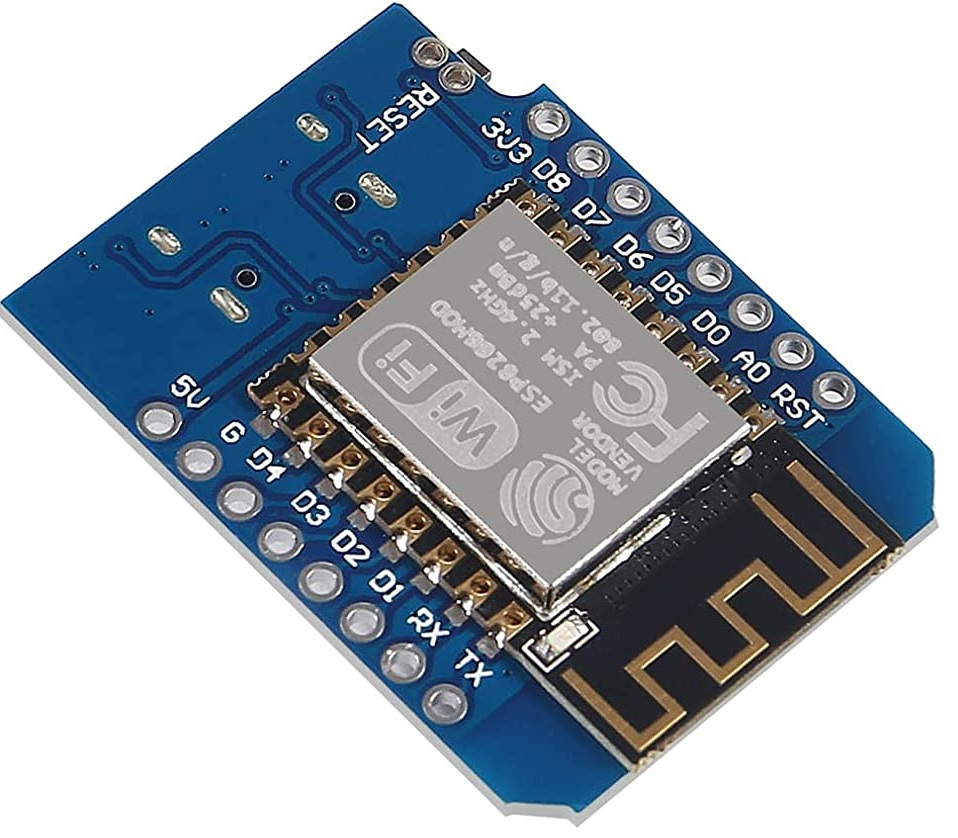
\includegraphics[width=0.60\textwidth]{./Figures/esp8266_2.jpg}
		\caption[Módulo de desarrollo ESP8266]{Módulo de desarrollo ESP8266.}
		\label{fig:esp8266}
     \end{subfigure}
     \hfill
        \caption[Módulos de desarrollo ESP empleados en el proyecto]{Módulos de desarrollo ESP empleados en el proyecto.}
        \label{fig:microESP}
\end{figure}





%\begin{figure}[h]
%	\centering
%	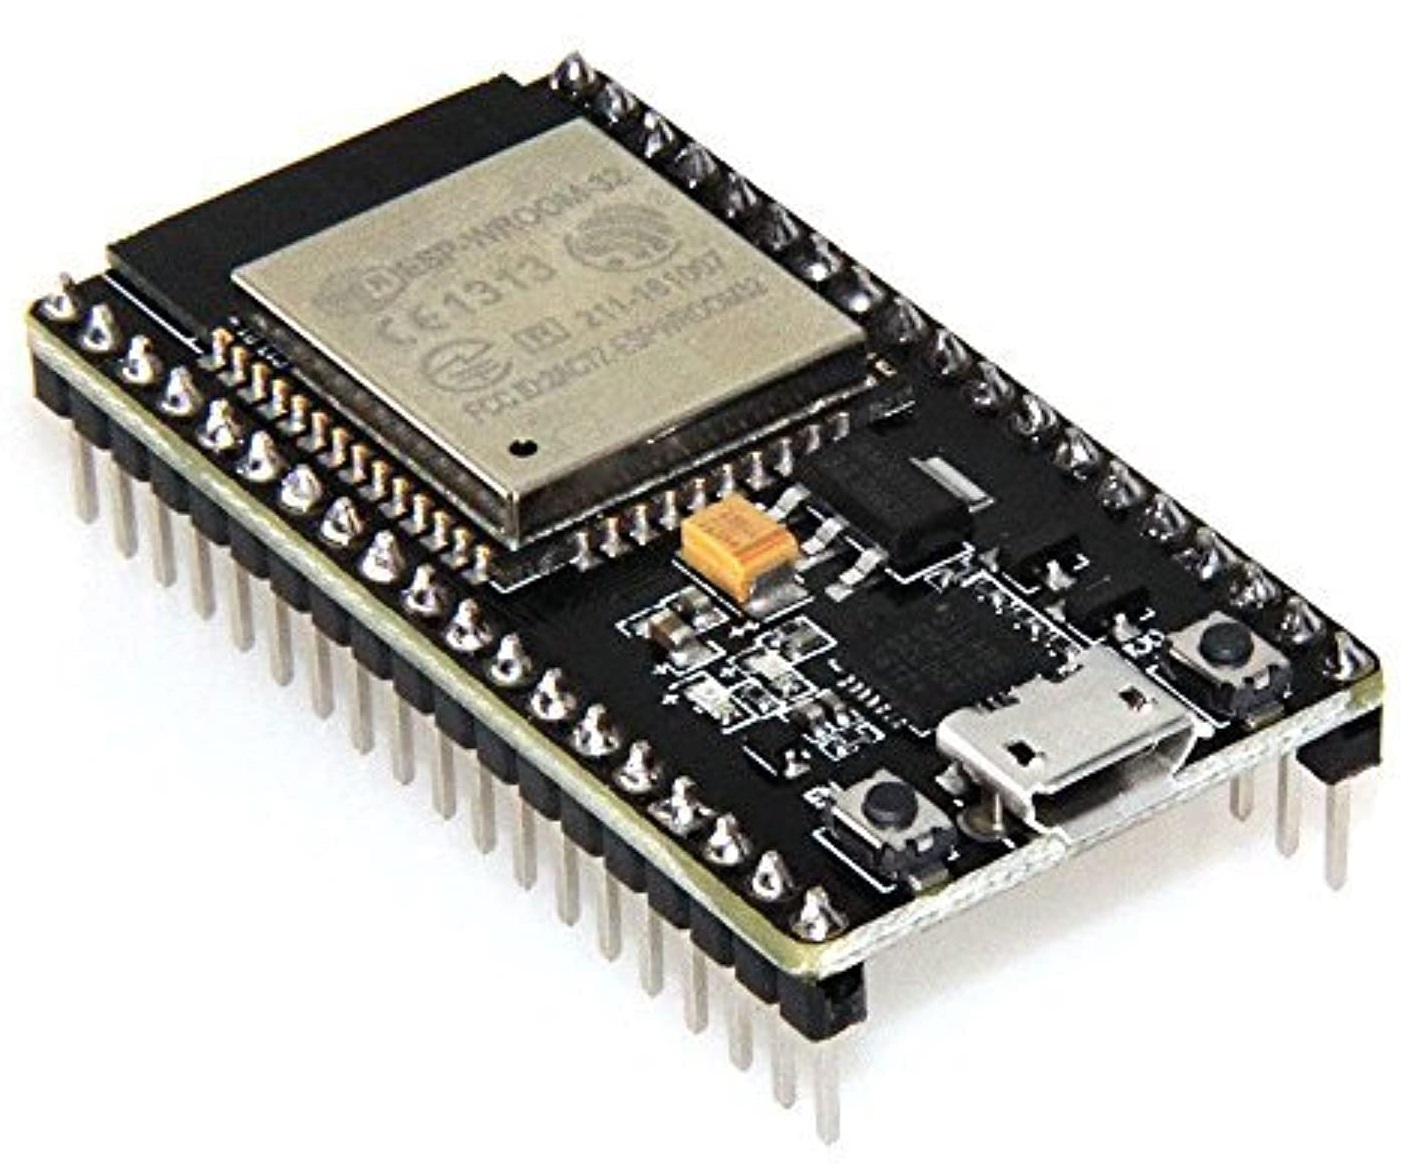
\includegraphics[width=0.30\textwidth]{./Figures/esp32.jpg}
%	\caption[Módulo de desarrollo ESP32.]{Módulo de desarrollo ESP32.}
%	\label{fig:esp32}
%
%\end{figure}


\subsection{Sensores y actuadores}
\label{sec:Sensores y actuadores}
Los principales sensores y actuadores empleados en el sistema del invernadero inteligente son los siguientes:
\begin{itemize}

\item DHT22: módulo básico y económico para determinar los valores de temperatura y humedad en forma digital. Utiliza un sensor de humedad capacitivo y un termistor para medir la temperatura en el aire circundante y entrega una señal digital en el pin de datos de acuerdo al valor calculado. Funciona con una alimentación de 3,3 a 6 VDC y su rango de medición es de -40 °C a 80 °C y de 0 a 100 \% de humedad relativa \citep{dht22}.

\item Sensor capacitivo de humedad del suelo: módulo analógico compuesto de un material resistente a la corrosión que mide la humedad del suelo indirectamente por medio de la capacitancia observada. Opera con una alimentación de 3,3 a 5,5 VDC y entrega un valor de tensión que varía entre 0 V para un suelo seco a aproximadamente 3,15 V en un suelo completamente húmedo \citep{soilsensor}.

\item Válvula solenoide de dos vías: dispositivo neumático para controlar el flujo de líquidos o gases que se acciona eléctricamente. Para poder operarla, se utiliza un relé que es un instrumento electromecánico que actúa como interruptor controlado por un circuito eléctrico \citep{valve}\citep{rele}.

La figura \ref{fig:sensores} muestra imágenes de los componentes listados previamente.

\end{itemize}
%\begin{figure}[h]
%	\centering
%	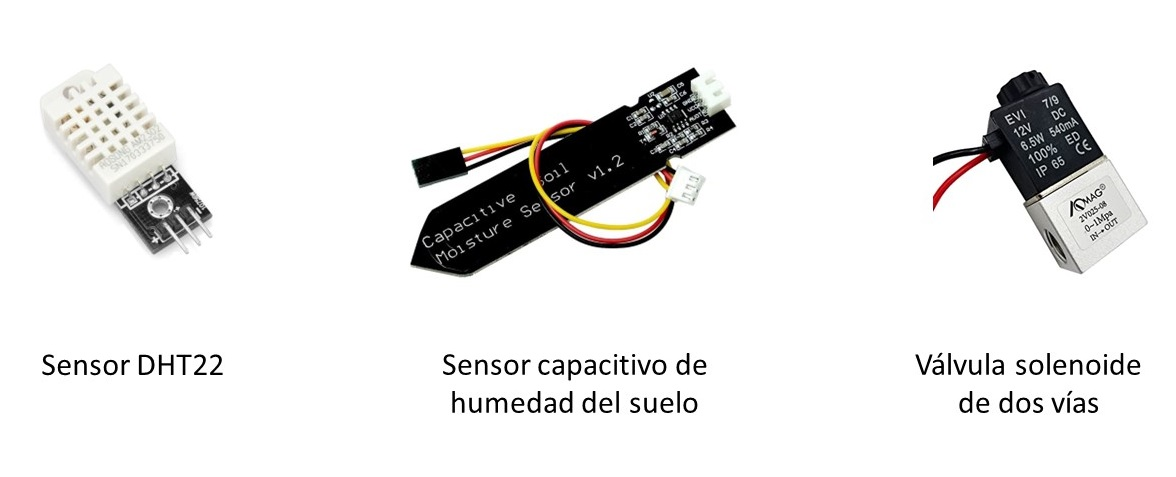
\includegraphics[width=0.90\textwidth]{./Figures/sensores.jpg}
%	\caption[Principales sensores y actuadores empleados en el invernadero.]{Principales sensores y actuadores empleados en el invernadero.}
%	\label{fig:sensores}
%
%\end{figure}

\begin{figure}[!htpb]
     \centering
     \begin{subfigure}[b]{0.3\textwidth}
         \centering
         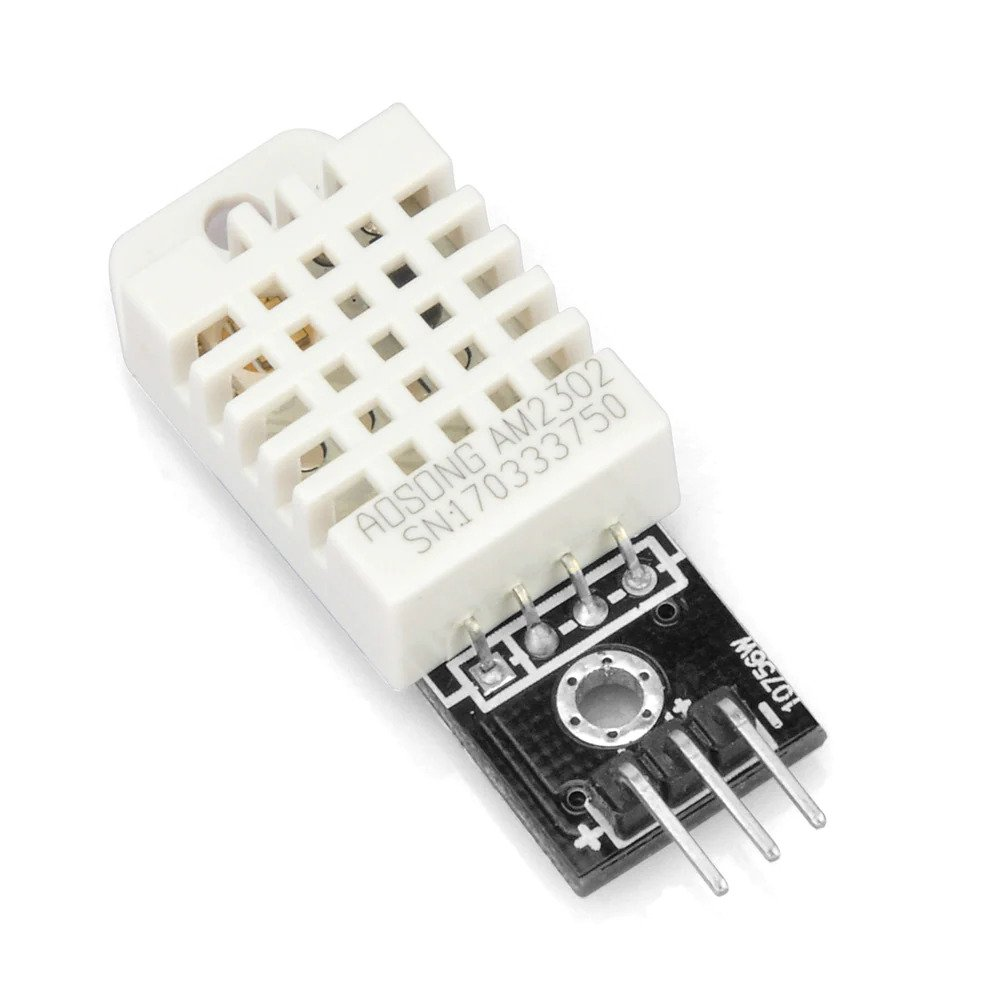
\includegraphics[width=.65\textwidth]{./Figures/dht22.jpg}
         \caption{Sensor de temperatura y humedad.}
         \label{fig:dht22}
     \end{subfigure}
     \hfill
     \begin{subfigure}[b]{0.3\textwidth}
         \centering
         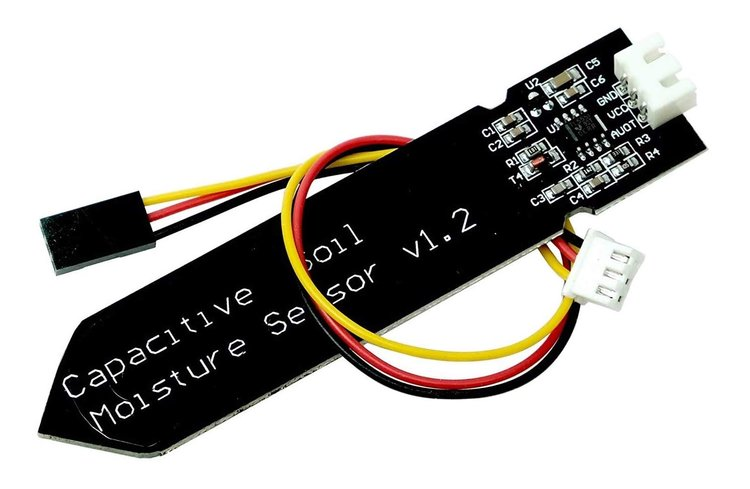
\includegraphics[width=.65\textwidth]{./Figures/soilsensor}
         \caption{Sensor de humedad del suelo.}
         \label{fig:soilsensor}
     \end{subfigure}
     \hfill
     \begin{subfigure}[b]{0.3\textwidth}
         \centering
         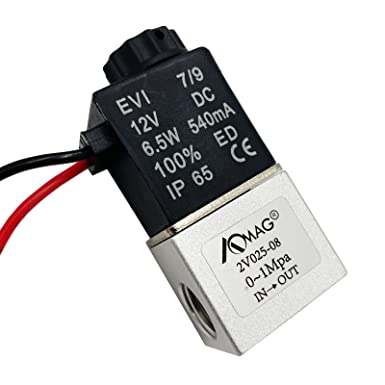
\includegraphics[width=.65\textwidth]{./Figures/valve.jpg}
         \caption{Válvula solenoide de dos vías.}
         \label{fig:valve}
     \end{subfigure}
        \caption[Principales sensores y actuadores empleados en el invernadero]{Principales sensores y actuadores empleados en el invernadero.}
        \label{fig:sensores}
\end{figure}




\section{Tecnologías de software aplicadas}
\label{sec:Software aplicado}
\subsection{ThingsBoard}
\label{sec:ThingsBoard}
ThingsBoard es una plataforma de código abierto que permite el desarrollo, administración y expansión de proyectos de IoT. Esta aplicación permite la gestión de las comunicaciones, el almacenamiento y la visualización de los datos que provienen de los sensores u otros dispositivos que forman parte del sistema \citep{thingsboard:1}.
Se ofrece en las siguientes versiones:
\begin{itemize}

\item Professional Edition: es la versión comercial, con varios tipos de licenciamiento y costos según sea el sistema a implementar. Esta edición posee soporte técnico, ilimitada cantidad de dispositivos a conectar y soporte para almacenamiento híbrido entre otras funcionalidades.

\item Cloud: similar a la edición profesional, pero alojada en la nube de ThingsBoard. En este caso el proveedor se encarga del manejo de los componentes de la plataforma.
 
\item Community edition: se encuentra bajo licencia Apache 2.0 \citep{apache2.0} y  es la que se utilizó en este trabajo. Si bien no tiene limitaciones en cuanto a la cantidad de dispositivos a conectar, carece de ciertas funcionalidades como por ejemplo la descarga de datos de dispositivos desde la interfaz web o la ejecución programada de tareas (\textit{scheduler}).
\end{itemize}
%
%\begin{table}[h]
%\centering
%\caption[Comparación de versiones de ThingsBoard]{Especificaciones técnicas de Raspberry PI 4B}
%
%\begin{tabular}{p{0.30\textwidth} p{0.15\textwidth} p{0.15\textwidth} p{0.15\textwidth}} 
%\toprule
%\textbf{Categoría} & \textbf{Community Edition} & \textbf{Professional Edition} & \textbf{Cloud}\\
%
%\midrule
%Gestión de activos y recopilación de datos				&	Sí &	Sí &	Sí\\
%Paneles de control en tiempo real para usuarios finales &	Sí &	Sí &	Sí\\
%Cadenas de reglas personalizables, widgets				&	Sí &	Sí &	Sí\\
%Transporte MQTT, HTTP, CoAP, OPC-UA						&	Sí &	Sí &	Sí\\
%Integraciones con sistemas BigData						&	Sí &	Sí &	Sí\\
%Soporte NB-IoT, SigFox, LoRaWAN				&	Sí &	Sí &	Sí\\
%Motor de reglas							& Básico & Avanzado & Avanzado\\
%Grupos de entidades										& Básico & Avanzado & Avanzado	\\	
%RBAC avanzado para IoT									&	No & Sí & Sí\\
%\textit{Scheduler}										&	No & Sí & Sí	\\
%Reportes												&	No & Sí & Sí\\
%Personalización de marca								&	No & Sí & Sí\\
%Exportación de datos							&	No & Sí & Sí\\
%Integraciones								&	No & Sí & Sí\\
%Gestión de dominios										&	No	& No & No\\
%\bottomrule
%\hline
%\end{tabular}
%\label{tab:raspberrypi}
%\end{table}

\subsection{Arduino IDE}
\label{sec:Arduino IDE}

Arduino IDE (\textit{Integrated Development Environment}) es un software de código abierto que se utiliza para escribir y cargar código a placas Arduino. Sin embargo por medio de la instalación de paquetes de expansión, el IDE soporta hardware de terceros entre los que encuentran las módulos ESP32/ESP8266 \citep{Arduinosupport} empleados en este proyecto.

El código de los programas se realiza en lenguaje C o C++ y los archivos resultantes se denominan \textit{sketches}. Estos son compilados y cargados en las placas desde el mismo IDE \citep{arduinoide}.

Este software es una herramienta fácil de utilizar tanto por usuarios experimentados como por principiantes. Es frecuentemente empleada por aquellos que se inician en la programación electrónica y la robótica o al momento de construir prototipos interactivos \citep{arduinoide:2}. 

\subsection{Telegram}
\label{sec:Telegram}

Telegram es una aplicación de mensajería multiplataforma rápida, simple y gratuita. Está basada en la nube y cuenta con sincronización constante, lo que significa que se puede acceder a los mensajes desde diferentes dispositivos simultáneamente. 

Tanto el código de los clientes de Telegram como el de su API tienen licencias abiertas, lo que permite crear otras aplicaciones a partir de ellos. Adicionalmente cuenta con una API para \textit{bots} que facilita la implementación de herramientas basadas en Telegram, la integración de servicios o la realización pagos \citep{telegram}.
 
  

\section{Requerimientos}
\label{sec:Requerimientos}

A continuación se listan los principales requerimientos funcionales,  no funcionales y de documentación del proyecto:

\begin{itemize}
\item Requerimientos funcionales:
\begin{enumerate}

\item El estado del sistema podrá ser consultado desde Internet.
\item La aplicación soportará múltiples usuarios de forma concurrente.
\item La aplicación permitirá crear roles de usuarios con diferentes permisos.
\end{enumerate}
\end{itemize} 
\begin{itemize}
\item Requerimientos no funcionales:
\begin{enumerate}
\item El rango de tensión de alimentación de los nodos será de 3,3 a 5 VDC.
\item El sistema de riego operará con una tensión de alimentación de 12 VDC.
\item La aplicación estará basada en software de código abierto.
\item El firmware deberá desarrollarse en plataformas de código abierto.
\item El trabajo se realizará sobre dispositivos de bajo costo y fácil reposición.
\item Los datos se almacenarán localmente.
\item La aplicación soportará MQTT.
\item Los sensores de humedad del suelo tendrán una protección similar a IP65 \citep{ip65}. 
\end{enumerate}


\end{itemize} 
\begin{itemize}
\item Requerimientos de documentación:
\begin{enumerate}
\item Los manuales y/o guías estarán redactados en inglés.
\end{enumerate}


\end{itemize}
